\subsubsection{Wersja YAML}
Finalną wersję pipeline'a umieściłem bezpośrednio w repozytorium jako pliki YAML w folderze \verb|CI|.
Korzystając z możliwości Azure podzieliłem duży plik zawierający wszystkie kroki 
na pomniejsze template'y (szablony), które mogę ponownie wykorzystać w dowolnie dużej 
ilości i kolejności.

Cała struktura zadań podzielona jest na kilka grup - tworząc je możemy zacząć od etapów (ang. stage), 
wewnątrz nich zawrzeć kilka jobów (prac, zadań), które składają się z kroków wykonania (ang. steps).


\begin{figure}[ht]
    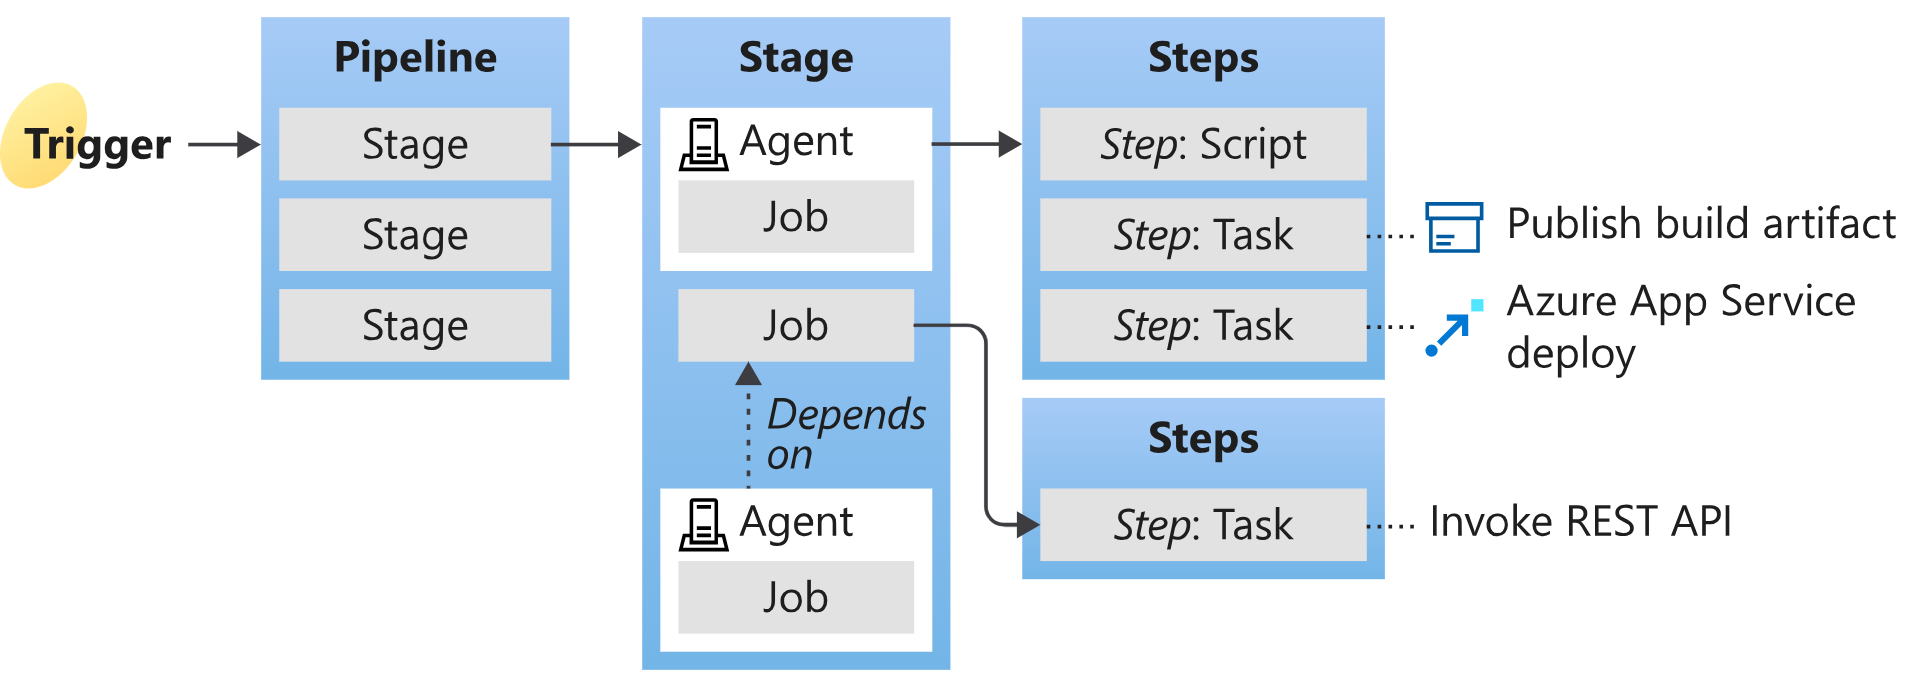
\includegraphics[width=\textwidth]{pipelineSchemaAzure.png}
    \caption{Hierarchia etapów i zadań w Azure~\cite{pipelineSchemaAzure_source}}
    \label{img:pipelineSchemaAzure}
    
\end{figure}

\subsubsection{Opis najciekawszych zadań z pipeline'a}

W tej sekcji opiszę moim zdaniem najciekawsze przypadki użycia zadań, które zastosowałem 
w mojej pracy. Pozwolę sobie pominąć przykładowo \verb|NuGetToolInstaller|, ponieważ użyłem 
go w sposób standardowy (wybrałem gotowe opcje z listy), nie powodował on większych problemów
ani istotniejszych przemyśleń.

\paragraph{Etap "Environment preparation" - przygotowanie środowiska}

\subparagraph{JavaToolInstaller} \label{javaTask}
To zadanie jest szczególnie ciekawe pod względem sposobu działania - aby uniknąć każdorazowego 
pobierania plików Java SDK lub wskazywania lokalnie pobranego pakietu, wygodnym dla mnie 
rozwiązaniem okazało się skorzystanie z parametru \verb|jdkSourceOption| o wartości \verb|PreInstalled|.
W oficjalnej dokumentacji~\cite{jdkSourceOption} możemy przeczytać, że za jej pomocą możemy skorzystać 
z preinstalowanej wersji JDK na Agentach udostępnianych przez Microsoft.

Jednak po wczytaniu się w temat udało mi się natrafić na odpowiedź~\cite{javaToolInstaller_StackOverflow}
użytkownika "R. Oosterholt", który wskazuje konwencję odnalezienia narzędzia, której używa zadanie.
Okazuje się, że jest to wskazanie ścieżki plików za pomocą systemowej zmiennej środowiskowej w określonym 
układzie nazewniczym.

Wywołanie zadania automatycznie udostępnia odnalezione programy do aktualnie wykonywanego etapu, dzięki czemu 
możemy użyć ich w kolejnych czynnościach.

\paragraph*{Etap "Compilation"}
\subparagraph{AndroidSigning}
Podpisywanie skompilowanego pliku \verb|.apk| okazało się być większym problemem niż początkowo przypuszczałem.
.NET MAUI oferował opcję automatycznego podpisania opublikowanej aplikacji, co wymagało podania jego szczegółów 
bezpośrednio w pliku projektu lub bezpośrednio w wywołaniu \verb|dotnet publish|.
Uznałem że lepszą opcją będzie skorzystanie z odrębnego zadania, co poskutkowało również skorzystaniem z opcji 
ZipAlign, który zmniejsza rozmiar pakietu oraz ilość zużywanej pamięci RAM.